\documentclass[../main.tex]{subfiles}
\begin{document}

\chapter{Parametric curves and splines}
\label{chp:parametriccurves}

Parametric curves are curves defined in a vector space by a parametric equation,
which can be as simple as a parabola or a circle. In an n-dimensional space,
these functions are often defined by one input — most commonly $t$ or $u$,
limited to the interval $[0, 1]$ — and $n$ outputs. Each of the $n$ coordinates
is its own independent function, and the combination of multiple coordinates
creates a curve, plane, or hyperplane.

Splines are a special kind of parametric curve that are defined as piecewise
polynomials and are most often used to interpolate between a set of points.

For the purpose of mobile robot path design, the most appropriate types of
splines are Bezier curves, B-splines, and NURBS curves. What these three models
have in common is that each curve is defined by its degree, a set of control
points in n-dimensional space and its basis functions. The position for a given
$t$ is a weighted sum of the curve's points, the weights being given by its
basis functions. In other words, the curve interpolates between all of its given
points.

In literature, the terms \emph{degree} and \emph{order} are both used to
describe polynomial curves and splines. While these terms are very closely
linked they are not interchangeable. The term \emph{degree} is most commonly
used in mathematical literature because it describes the actual degree of the
curve's polynomial. The term \emph{order}, on the other hand, is used in CAGD
literature and describes the order of continuity along the curve, which is more
relevant than the degree of the polynomial in engineering. The degree is always
equal to the order minus one. The term \emph{degree} will be used going forward
for consistency.

\section{Bezier}

Bezier curves are the simplest of the three. The most commonly used types of
Bezier curves are quadratic and cubic curves, defined by three and four points
respectively. The degree of a Bezier curve is always equal to the number of
control points minus one.

\begin{equation}
    C(u) = \sum_{i=0}^{n}B_{i,n}(u)P_i
\end{equation}

A Bezier curve's basis functions, or blending functions, are known as Bernstein
polynomials. There are $n+1$ basis functions for a curve of the n-th degree.
\cite{primer} In other words, there are as many polynomials as there are control
points. Bernstein polynomials are defined only by the curve's degree, meaning
that all Bezier curves of the same degree have the exact same Bernstein
polynomials.

\begin{equation}
    B_{i,n}(u) = \frac{n!}{i!(n-i)!} u^i (1-u)^{n-i}
\end{equation}

\begin{figure}[h]
    \centering
    \begin{tikzpicture}
        \begin{groupplot}[
            group style={
                group size=3 by 1,
                horizontal sep=0.8cm,  % No gap between plots
                },
            width=0.36\textwidth,
            height=5cm,
            axis y line=left,  % Only left side has y-axis
            axis x line=bottom,
            xlabel = \(t\),
            ymin=0, ymax=1,
        ]
        
        \nextgroupplot[ylabel={\(B(t)\)}]
        \addplot [domain=0:1,samples=100] {1-x};
        \addplot [domain=0:1,samples=100] {x};
        
        \nextgroupplot
        \addplot [domain=0:1,samples=100] {(1-x)^2};
        \addplot [domain=0:1,samples=100] {2*x*(1-x)};
        \addplot [domain=0:1,samples=100] {x^2};
        
        \nextgroupplot
        \addplot [domain=0:1,samples=100] {(1-x)^3};
        \addplot [domain=0:1,samples=100] {3*x*(1-x)^2};
        \addplot [domain=0:1,samples=100] {3*x^2*(1-x)};
        \addplot [domain=0:1,samples=100] {x^3};
        
        \end{groupplot}
    \end{tikzpicture}
    \caption{Basis functions for a Bezier curve of degree 1, 2 and 3}
    \label{fig:bezier_bernstein}
\end{figure}

Figure \ref{fig:bezier_bernstein} shows three examples of Bernstein polynomials,
for a Bezier curve of degrees 1, 2 and 3 respectively. This shows how a given
curve has as many Bernstein polynomials as there are control points, and each
polynomial represents the influence that a control point has on the curve at a
given parameter $t$. A Bernstein polynomial must be non-zero across the whole
parameter range of $ \left[0,1\right] $, meaning that all control points have
influence over the entire curve. This makes Bezier curves unsuitable for
defining long, continuous paths as they do not have \emph{local control}. Local
control is defined as the ability to modify a specific part of a curve without
affecting the rest of the curve.

\section{B-spline}

B-splines, short for “basis splines,” are a generalization of Bezier curves.
Unlike Bezier curves, which have static basis functions dependent on degree, the
basis functions of a B-spline can be modified using what is called a knot
vector. The number of control points on a B-spline is arbitrary and not
dependent on its degree, unlike Beziers.

We call B-splines \emph{piecewise polynomial} splines because they are composed
of a series of polynomial segments. This is different from Bezier curves which
are, by definition, a single polynomial.

\begin{equation}
    C(u) = \sum_{i=0}^{n}B_{i,n}(u)P_i
\end{equation}

The basis functions of a B-spline are not necessarily non-zero in the entire
range $\left[0, 1\right] $, meaning that a given basis function may not have influence on
the entire curve, i.e. a given point on the curve may not be defined by all of
its control points. This makes it possible to create complex shapes using a
single B-spline.

\begin{equation}
\begin{aligned}
    B_{i,p}(t) &= \frac{t - t_i}{t_{i+p} - t_i} B_{i,p-1}(t) + 
    \frac{t_{i+p+1} - t}{t_{i+p+1} - t_{i+1}} B_{i+1,p-1}(t) \\
    B_{i,0}(t) &= \begin{cases}
  1 & t_i \leq t < t_{i+1}\\
  0 & \text{otherwise}
\end{cases}
\end{aligned}
\end{equation}

A B-spline of degree $p$ and with $N$ control points has a knot vector of size
$N+p+1$. Each control point affects $p$ knots. By moving a knot's value up or
down, we can make a section of the curve denser in control points while making
the rest more sparse. Each span between two knots, i.e. between two values of
$t$, can be seen as a separate curve controlled by $p+1$ points, much like a
Bezier. However, this is a much better solution than chaining Bezier curves
because the model guarantees geometric continuity between knot spans, while a
chain of Beziers needs to be adjusted manually to be continuous.

\begin{figure}[h]
    \centering
    \begin{tikzpicture}
        \begin{axis}[
            width=15cm,
            height=8cm,
            xlabel={$t$},
            ylabel={Basis Function Value},
            xmin=0.0, xmax=1.0,
            ymin=-0.0, ymax=1.0,
            grid=both,
            grid style={line width=.1pt, draw=gray!10},
            major grid style={line width=.2pt,draw=gray!50},
            legend pos=north east,
            legend cell align=left,
            samples=100,
            smooth,
            line width=1.5pt,
            title={$\mathbf{T}=\begin{bmatrix} 0 & 0 & 0 & 0.25 & 0.5 & 0.75 & 1 & 1 & 1 \end{bmatrix}$},
        ]

        % Basis function N_{0,2}(t)
        \addplot[red, domain=0.0:0.25] {1 - 8*x + 16*x^2};

        % Basis function N_{1,2}(t)
        \addplot[blue, domain=0.0:0.25] {8*x - 24*x^2};
        \addplot[blue, domain=0.25:0.5] {2 - 8*x + 8*x^2};

        % Basis function N_{2,2}(t)
        \addplot[green!70!black, domain=0.0:0.25] {8*x^2};
        \addplot[green!70!black, domain=0.25:0.5] {-1.5 + 12*x - 16*x^2};
        \addplot[green!70!black, domain=0.5:0.75] {4.5 - 12*x + 8*x^2};

        % Basis function N_{3,2}(t)
        \addplot[orange, domain=0.25:0.5] {0.5 - 4*x + 8*x^2};
        \addplot[orange, domain=0.5:0.75] {-5.5 + 20*x - 16*x^2};
        \addplot[orange, domain=0.75:1.0] {8 - 16*x + 8*x^2};

        % Basis function N_{4,2}(t)
        \addplot[purple, domain=0.5:0.75] {2 - 8*x + 8*x^2};
        \addplot[purple, domain=0.75:1.0] {-16 + 40*x - 24*x^2};

        % Basis function N_{5,2}(t)
        \addplot[cyan!70!black, domain=0.75:1.0] {9 - 24*x + 16*x^2};

        % Knot positions
        \addplot[gray, dashed, forget plot] coordinates {(0.0,-0.05) (0.0,1.1)};
        \addplot[gray, dashed, forget plot] coordinates {(0.25,-0.05) (0.25,1.1)};
        \addplot[gray, dashed, forget plot] coordinates {(0.5,-0.05) (0.5,1.1)};
        \addplot[gray, dashed, forget plot] coordinates {(0.75,-0.05) (0.75,1.1)};
        \addplot[gray, dashed, forget plot] coordinates {(1.0,-0.05) (1.0,1.1)};

        \end{axis}
    \end{tikzpicture}
    \caption{Example basis functions for a quadratic B-spline}
    \label{fig:bspline_basisfunc}
\end{figure}

Figure \ref{fig:bspline_basisfunc} shows the basis functions of a uniform second
degree B-spline with six control points. Each basis function is drawn in a
different color, and the dashed vertical lines mark the edges between individual
knot spans. One thing that can be noticed in the graph is that each knot span
has exactly three "active" or non-zero basis functions at a time. Much like a
Bezier curve, each knot span of degree $p$ is controlled by $p+1$ points, but
B-splines differ from a chain of Bezier curves in the fact that the basis
functions are continuous from one span to another. A chain of Bezier curves can
only have the desired degree of geometric continuity if its control points are
placed in a specific manner, whereas a B-spline will be continuous across its
spans by definition.

One important property of B-splines, mentioned earlier, is that Bezier curves
are a subset of B-splines. By manipulating the knot vector, we can effectively
create a Bezier curve or a chain of Bezier curves from a single B-spline. Figure
\ref{fig:bspline_bezier} shows the basis functions of a quadratic B-spline with
six points and a knot vector of $\left[0 ~ 0 ~ 0 ~ 0.5 ~ 0.5 ~ 0.5 ~ 1 ~ 1 ~ 1\right]$. This
also shows how a knot with a multiplicity of $p+1$ results in a
non-differentiable peak.


\begin{figure}[h]
    \centering
    \begin{tikzpicture}
        \begin{axis}[
            title={$\mathbf{T}=\begin{bmatrix} 0 & 0 & 0 & 0.5 & 0.5 & 0.5 & 1 & 1 & 1 \end{bmatrix}$},
            width=15cm,
            height=8cm,
            xlabel={$t$},
            ylabel={Basis Function Value},
            xmin=0.0, xmax=1.0,
            ymin=-0.0, ymax=1.0,
            grid=both,
            grid style={line width=.1pt, draw=gray!10},
            major grid style={line width=.2pt,draw=gray!50},
            legend pos=north east,
            legend cell align=left,
            samples=100,
            smooth,
            line width=1.5pt,
        ]

        \addplot [red, domain=0:0.5,samples=100] {(1-x*2)^2};
        \addplot [blue, domain=0:0.5,samples=100] {4*x*(1-x*2)};
        \addplot [green!70!black, domain=0:0.5,samples=100] {(x*2)^2};

        \addplot [orange, domain=0.5:1,samples=100] {(1-2*(x-0.5))^2};
        \addplot [purple, domain=0.5:1,samples=100] {2*(2*(x-0.5))*(1-2*(x-0.5))};
        \addplot [cyan!70!black, domain=0.5:1,samples=100] {(2*(x-0.5))^2};

        % Knot positions
        \addplot[gray, dashed, forget plot] coordinates {(0.5,0.0) (0.5,1.0)};

        \end{axis}
    \end{tikzpicture}
    \caption{Basis functions of a B-spline equivalent to two chained Beziers}
    \label{fig:bspline_bezier}

\end{figure}

This is very close to what we want but it's still difficult to make sharp turns
and precise movements without increasing the degree of the curve, making it more
expensive to compute in real-time. It is possible to achieve even more control
over the shape of our curve using NURBS.

\section{NURBS}

NURBS curves are a further generalization of B-splines. The acronym stands for
“non-uniform rational basis spline.” \cite{Piegl_Tiller_1997}

\begin{equation}
    \mathbf{C}(u) = \sum_{i=1}^{n}\frac{B_{i,p}(u)w_i}{\sum_{j=1}^{n}B_{j,p}(u)w_j} \mathbf{P}_i
    = \sum_{i=1}^{n}R_{i, p}\mathbf{P}_i
\end{equation}

We describe NURBS as “non-uniform” because its basis functions do not need to be
uniformly distributed. This is done using a knot vector which defines the
distribution of a curve's basis functions. B-splines are also non-uniform, as
described earlier, though this is not reflected in the name.

We also describe NURBS as “rational” because they let us define a ratio, i.e., a
weight, for each control point. This means that we can define the influence that
a control point has on the overall curve. In terms of basis functions, this
effectively scales a particular basis function in relation to its neighboring
functions, creating a \emph{rational basis function} $R_{i, p}$. Another way to
interpret this is that all control points are defined in \emph{homogenous
coordinates}, using the three coordinates $x, y$ and $w$, with the resulting
spline being projected onto the plane $w=1$.

Both of the aforementioned parametric curve models are subsets of NURBS curves.
By limiting the parameters of a NURBS curve we can effectively create a Bezier,
a B-spline, or a rational Bezier, among other types of splines.

Much like B-splines, a NURBS curve of degree p and N control points has a knot
vector of size N+p+1 and each point affects p knots. Each basis function belongs
to one control point. Scaling a particular point's weight also scales its basis
function in comparison to its neighboring functions, however it can still only
reach the $p-1$ knot spans before and after it, maintaining local control.


\begin{figure}[h]
    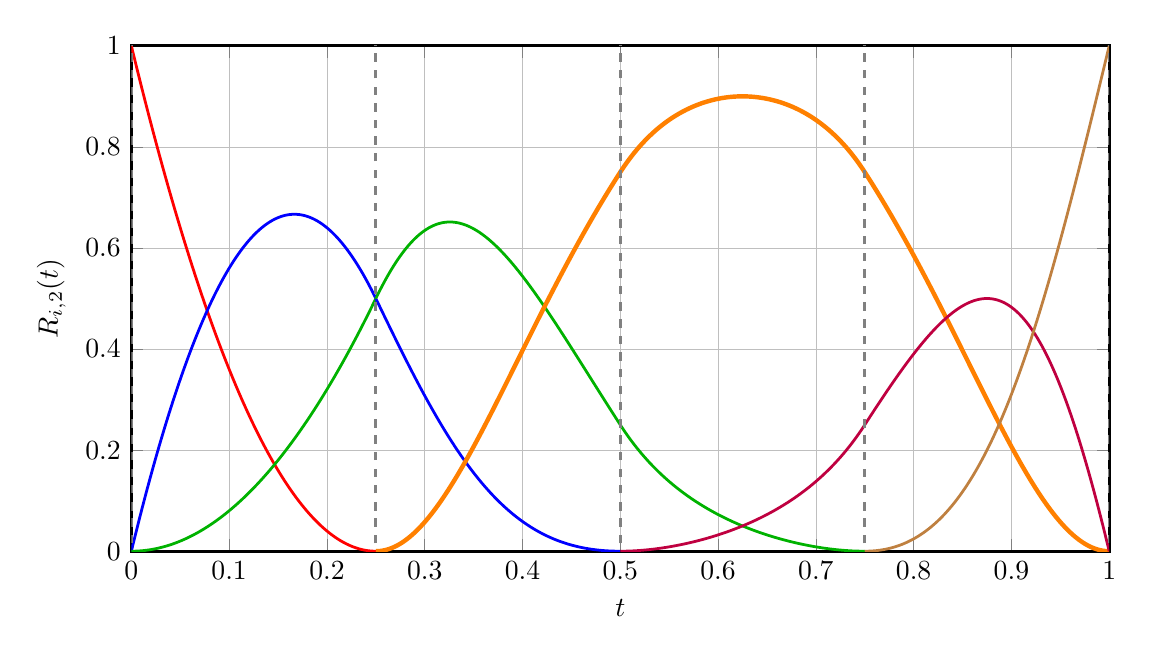
\begin{tikzpicture}
        \begin{axis}[
            width=14cm,
            height=8cm,
            xlabel={$t$},
            % ylabel={Rational Basis Function Value},
            ylabel={$R_{i, 2}(t)$},
            % title={NURBS Rational Basis Functions $R_{i,2}(t)$ with weights $[1,1,1,3,1,1]$},
            xmin=0.0, xmax=1.0,
            ymin=0.0, ymax=1.0,
            grid=both,
            grid style={line width=.1pt, draw=gray!10},
            major grid style={line width=.2pt,draw=gray!50},
            legend pos=north east,
            legend cell align=left,
            samples=200,
            smooth,
            line width=1.0pt,
        ]
        
        % NURBS Rational Basis Functions
        % Knot vector: [0, 0, 0, 0.25, 0.5, 0.75, 1, 1, 1]
        % Degree p = 2, Weights: w = [1, 1, 1, 3, 1, 1]
        
        \addplot[red, domain=0.0:0.25] {(1 - 8*x + 16*x^2)/1};
        \addplot[blue, domain=0.0:0.25] {(8*x - 24*x^2)/1};
        \addplot[green!70!black, domain=0.0:0.25] {(8*x^2)/1};
        \addplot[blue, domain=0.25:0.5] {(2 - 8*x + 8*x^2)/(2 - 8*x + 16*x^2)};
        \addplot[green!70!black, domain=0.25:0.5] {(-1.5 + 12*x - 16*x^2)/(2 - 8*x + 16*x^2)};
        \addplot[orange, ultra thick, domain=0.25:0.5] {3*(0.5 - 4*x + 8*x^2)/(2 - 8*x + 16*x^2)};
        \addplot[green!70!black, domain=0.5:0.75] {(4.5 - 12*x + 8*x^2)/(-10 + 40*x - 32*x^2)};
        \addplot[orange, ultra thick, domain=0.5:0.75] {3*(-5.5 + 20*x - 16*x^2)/(-10 + 40*x - 32*x^2)};
        \addplot[purple, domain=0.5:0.75] {(2 - 8*x + 8*x^2)/(-10 + 40*x - 32*x^2)};
        \addplot[orange, ultra thick, domain=0.75:1.0] {3*(8 - 16*x + 8*x^2)/(17 - 32*x + 16*x^2)};
        \addplot[purple, domain=0.75:1.0] {(-16 + 40*x - 24*x^2)/(17 - 32*x + 16*x^2)};
        \addplot[brown, domain=0.75:1.0] {(9 - 24*x + 16*x^2)/(17 - 32*x + 16*x^2)};
        % Knot positions
        \addplot[gray, dashed, forget plot] coordinates {(0,-0.05) (0,1.1)};
        \addplot[gray, dashed, forget plot] coordinates {(0.25,-0.05) (0.25,1.1)};
        \addplot[gray, dashed, forget plot] coordinates {(0.5,-0.05) (0.5,1.1)};
        \addplot[gray, dashed, forget plot] coordinates {(0.75,-0.05) (0.75,1.1)};
        \addplot[gray, dashed, forget plot] coordinates {(1.0,-0.05) (1.0,1.1)};
        
        \end{axis}
    \end{tikzpicture}
    \label{fig:nurbs_weighted_bf}
    \caption{Example basis functions for a quadratic NURBS, with one point weighted}
\end{figure}

A NURBS curve of degree p always has geometric continuity of the $(p-1)$-th
degree along its length. Changing the knot vector may affect this property if
there are multiple identical knots inside the curve. Each duplicate knot reduces
the geometric continuity in that point by 1. Having $p$ identical knots in the
knot vector results in a sharp peak which only has $G^0$ continuity. All of this
should be avoided, or prohibited to the end-user, if the goal is to maintain
geometric continuity. Adjusting the weights cannot affect geometric continuity
in any case.

\subsection{Conic sections}

One property of NURBS that is not applicable to Bezier curves and B-splines is
that they can represent conic sections, i.e., circles, ellipses and parabolas.
This is made possible by the ability to weigh specific points. \cite{farin1992from}

\subsection{Matrix representation of NURBS}

The general formula for NURBS evaluation can be expressed in the form of a
matrix making it more appropriate for programmatic computation. \cite{731996}

The basis matrix of a spline is defined recursively using Equation
\eqref{eq:basisfunc}. This matrix is applicable to both NURBS and B-splines due
to the fact that it depends only on the knot vector, which is a feature of both
NURBS and B-splines, and does not depend on weights which are exclusive to
NURBS. Equation \eqref{eq:basisfunc} calculates the $i$-th basis matrix, with
$i$ being the index of a particular knot span. The elements on the main and
first diagonal are calculated using Equation \eqref{eq:bf_elements}, with $t_i$
being the $i$-th element of the knot vector. For a knot span of degree $p$,
computing its basis matrix requires $i$ iterations with constant-time operations,
resulting in $\mathit{O(p)}$ time complexity.

\begin{equation}
    \label{eq:basisfunc}
    \begin{aligned}
    \mathbf{M}^{k}(i) &=
    \begin{bmatrix}
    \mathbf{M}^{k-1}(i)\\ \mathbf{0}
    \end{bmatrix}
    \begin{bmatrix}
    1-d_{0,i-k+2} & d_{0,i-k+2} &        & 0 \\
                  & 1-d_{0,i-k+3} & d_{0,i-k+3} \\
                  & \ddots        & \ddots \\
    0             &               & 1-d_{0,i} & d_{0,i}
    \end{bmatrix}
    \\
    &\quad +
    \begin{bmatrix}
    \mathbf{0} \\ \mathbf{M}^{k-1}(i)
    \end{bmatrix}
    \begin{bmatrix}
    - d_{1,i-k+2} & d_{1,i-k+2} & & 0 \\
                  & - d_{1,i-k+3} & d_{1,i-k+3} \\
                  & \ddots        & \ddots \\
    0             &               & - d_{1,i} & d_{1,i}
    \end{bmatrix}
    \\
    \mathbf{M}^1(i) &= \begin{bmatrix} 1 \end{bmatrix}
    \end{aligned}    
\end{equation}

\begin{equation}
    \label{eq:bf_elements}
    \begin{aligned}
        d_{0, j} &= \frac{t_i-t_j}{t_{j+k-1}-t_j} \\
        d_{1, j} &= \frac{t_{i+1}-t_i}{t_{j+k-1}-t_j}
    \end{aligned}
\end{equation}

A point on a knot span at a given parameter value $u$ is evaluated using
Equation \eqref{eq:nurbs_point}. Equation \eqref{eq:t_powseries} describes the
power series of the parameter value $u$, while Equation
\eqref{eq:nurbs_controlpts} describes the weighted control points and the
weights affecting the knot span. Given that the vector $\mathbf{U}^k$ has a size
of $1 \times k$, the matrix $\mathbf{M}^k$ a size of $k \times k$ and
$\mathbf{P}^k$ a size of $k \times n$, we can tell that the result is a point in
$n$-dimensional space. The denominator is always a scalar.

\begin{equation}
    \label{eq:nurbs_point}
    \begin{aligned}
        \mathbf{c}_{i-k+1}(u) &= \frac{\mathbf{U}^k\mathbf{M}^k(i)\mathbf{P}^k(i)}
                                      {\mathbf{U}^k\mathbf{M}^k(i)\mathbf{W}^k(i)} \\
                            &= \frac{\mathbf{R}(u)}{S(u)} 
    \end{aligned}
\end{equation}

\begin{equation}
    \label{eq:t_powseries}
    \mathbf{U}^k = \begin{bmatrix}
        1 & u & u^2 & \dots & u^{k-1}
    \end{bmatrix}
\end{equation}

\begin{equation}
    \label{eq:nurbs_controlpts}
    \mathbf{P}^k(i) = \begin{bmatrix}
        w_{i-k+1}\mathbf{V}_{i-k+1} \\
        w_{i-k+2}\mathbf{V}_{i-k+2} \\
        \vdots \\
        w_{i}\mathbf{V}_{i} \\
    \end{bmatrix} ,
    \mathbf{W}^k(i) = \begin{bmatrix}
        w_{i-k+1} \\
        w_{i-k+2} \\
        \vdots \\
        w_{i} \\
    \end{bmatrix}
\end{equation}

With the basis function, control points and weights all being known constants,
evaluating a point on a knot span only requires computing the vector
$\mathbf{U}^k$ and performing the necessary matrix multiplication instead of the
iterative sum given by the original definition of NURBS.

\subsection{Derivative calculation}

Knowing that the matrices $\mathbf{M}$, $\mathbf{P}$ and $\mathbf{W}$ are
independent of $\mathbf{U}$, we can calculate the derivative of Equation
\eqref{eq:nurbs_point} as given in equation \eqref{eq:nurbs_derivative}.

\begin{equation}
    \label{eq:nurbs_derivative}
    \frac{d^n}{dt^n} \mathbf{c}_{i-k+j}(u) = 
    \sum_{j=0}^{n} \binom{n}{j} \frac{d^j}{dt^j} \{\mathbf{R}(u)\} \cdot 
    \frac{d^{n-j}}{dt^{n-j}} \{1/S(u)\}
\end{equation}

We know from Equation \ref{eq:nurbs_point} that $\mathbf{R}(u)$ is equal to
$\mathbf{U^k}\mathbf{M^k}(i)\mathbf{P^k}(i)$. Differentiating $\mathbf{R}(u)$
involves only differentiating the elements of the vector $\mathbf{U}^k$ by $u$,
since the other elements are constants independent of $u$. Differentiating
$1/S(u)$ requires the quotient rule.

\subsection{Curvature and curvature derivative}

Equation \ref{eq:curvature} defines the curvature of a parametric curve at a
parameter $t$. This value represents the inverse of the radius of a circle that
can be inscribed inside the curve; a straight line has a curvature of infinity.
This formula is not specific to NURBS but can be applied to any
twice-differentiable parametric curve, or thrice-differentiable for the
derivative.

\begin{equation}
    \label{eq:curvature}
    \kappa(t) = \frac{\mathbf{c}'(t)\times \mathbf{c}''(t)}{\left\lVert \mathbf{c}'(t) \right\rVert^3 }
\end{equation}

\begin{equation}
    \label{eq:curvature_derivative}
    \frac{d}{dt} \kappa(t) = \frac{\mathbf{c}'(t)\times \mathbf{c}'''(t)}{\left\lVert \mathbf{c}'(t) \right\rVert^3 }
    - 3\left(\mathbf{c}'(t)\cdot \mathbf{c}''(t)\frac{\mathbf{c}'(t)\times \mathbf{c}''(t)}{\left\lVert \mathbf{c}'(t) \right\rVert^5 }\right) 
\end{equation}

\subsection{Curve splitting}

Splitting a NURBS curve at a given parameter $t$ amounts to splitting whichever
one of its knot spans contains the point $t$. Using matrix notation, splitting a
knot span into two separate spans is straightforward.

% \begin{equation}
%     \mathbf{L}_{p}(t) = \begin{bmatrix}
%         1 &  &  &  & 0\\
%          & t &   &  \\
%          & & t^2 &  \\
%          &  &  &  \ddots & \\
%         0 &  &  &  &  t^p\\
%     \end{bmatrix}
% \end{equation}

% \begin{equation}
%     \mathbf{R}_{p}(t) = \begin{bmatrix}
%         1 &  &  &  & 0\\
%          & t &   &  \\
%          & & t^2 &  \\
%          &  &  &  \ddots & \\
%         0 &  &  &  &  t^p\\
%     \end{bmatrix}
% \end{equation}

\section{Comparison of NURBS, B-splines and Bezier curves}
\label{chp:comparison}

Most software using parametric curves primarily uses Bezier curves, however they
are limited in their capabilities. In some fields such as graphic design this is
not considered a problem, as their simplicity and computation speed are more
valuable than highly precise shapes. Other fields, such as engineering or
robotics, require highly optimized and precise paths, for which Bezier curves
are often not sufficient. Software meant for engineering and CAGD, such as
AutoCAD and Rhino, use NURBS for this reason.

Out of the three curve models presented, NURBS are the most flexible and allow
for the most control, though they might be computationally expensive. However,
having modifiable weights gives us a level of flexibility above B-splines
without increasing the degree, which makes them potentially more efficient than
B-splines if used wisely.

Because all B-splines can be expressed as a NURBS curve with all weights set to $1.0$,
and all Bezier curves can be expressed as a B-spline with knot multiplicity, it
can be concluded that NURBS are a superset of both B-splines and Bezier curves.
By implementing NURBS it is possible to cover all use cases of the other two
parametric curve types, as well as providing additional flexibility.

\end{document}